% !TEX program = xelatex
\documentclass[aspectratio=169]{ctexbeamer}
\usetheme{CambridgeUS}
\setbeamertemplate{navigation symbols}{}
\usepackage{amsmath, amssymb}
\usepackage[en-US]{datetime2}
% \usepackage{enumitem}
\usepackage{pgf, tikz}
\usetikzlibrary{positioning}
\tikzset{
    rednode/.style={
        circle,
        draw=red, % 边框颜色为红色
        fill=red!10, % 填充颜色为红色的 10%
        thick, % 边框加粗
        minimum size=0.75cm,
        inner sep=0,
        font=\bf\small
    },
    bluenode/.style={
        circle,
        draw=blue,
        fill=blue!10,
        thick, % 边框加粗
        minimum size=0.75cm,
        inner sep=0,
        font=\bf\small
    }
}
\usepackage{caption}
\usepackage{subcaption}
\captionsetup{labelfont=bf, labelsep=quad, font=footnotesize}
\renewcommand{\figurename}{Figure}
\renewcommand{\tablename}{Table}
\usepackage{booktabs}
\usepackage[algoruled, linesnumbered]{algorithm2e}
\SetKwProg{Function}{Function}{}{end}
\SetFuncSty{textsc}
\SetArgSty{}
\SetFuncArgSty{}
\algomargin=1em
\SetNlSty{textbf}{}{:}
\DontPrintSemicolon
\usepackage{calligra}
\usepackage{listings}
\lstset{
    language = C++,
    breaklines = true,
    extendedchars = false,  % 解决代码跨页时,章节标题,页眉等汉字不显示的问题
    basicstyle = \ttfamily,
    keywordstyle = \bfseries,
    numbers = left,
    numberstyle = \small,
    frame = single,
    backgroundcolor = \color{lightgray!40!white},
    showstringspaces = false,
    tabsize = 4,
    commentstyle = \it\color{gray},
    xleftmargin = 1em,
}
\title{Day 8: Data Structures II}
\subtitle{Binary Heaps \& Disjoint-Set Forests}
\author{Tinghai Zhang}
\date{Jan 9, 2025}
\newcommand{\highlight}[1]{\textbf{\textit{#1}}}
\renewcommand{\leq}{\leqslant}
\renewcommand{\geq}{\geqslant}
\hypersetup{
    pdftitle = {Day 8: Binary Heaps and Disjoint-Set Forests},
    pdfauthor = {Tinghai Zhang},
    pdfsubject = {Data Structures},
    pdfkeywords = {binary heaps, disjoint-set forests},
    pdfpagemode = FullScreen
}
\begin{document}
    \begin{frame}
        \maketitle
    \end{frame}

    \section{Binary heaps}

    \subsection{Priority queue ADT}

    \begin{frame}{Priority queue ADT}{Requirements}
        There are some items with \highlight{priority}, and we need an ADT which supports:

        \begin{itemize}
            \item The next item to access or remove is the \highlight{highest-priority} item.
            \item New items may be added \highlight{any time}.
        \end{itemize}

        One of common use cases: hospital emergency department.
    \end{frame}

    \begin{frame}{Priority queue ADT}{Two basic implementation}
        \begin{itemize}
            \item (Unsorted) array
            \begin{itemize}
                \item Enqueue: add new item at the end of the array, $\mathcal O(1)$.
                \item Dequeue: scan the array to find the highest-priority item, $\mathcal O(n)$.
            \end{itemize}
            \item Sorted array
            \begin{itemize}
                \item Enqueue: scan the array to find the right position for the new item, $\mathcal O(n)$.
                \item Dequeue: remove the last item, $\mathcal O(1)$.
            \end{itemize}
        \end{itemize}
    
        Entirely unsorted is too chaotic, but entirely sorted is unnecessary. A compromise is to use a \highlight{heap}.
    \end{frame}

    \subsection{Binary heaps}

    \begin{frame}{Binary heaps}{Definition}
        \highlight{Binary heaps} store items \highlight{partially sorted}. All the items are stored in a \highlight{binary tree}, which satisfies:
        \begin{itemize}
            \item The tree is \highlight{complete}, i.e. nodes in it are filled left-to-right on each level (row) of the tree.
            \begin{itemize}
                \item The tree is complete if and only if the array representation of the tree is filled from index 0 to $n-1$.
            \end{itemize}
            \item The tree is \highlight{heap-ordered}, i.e. the value of each node is \highlight{greater than or equal to} the values of its children. We call the property \highlight{max-heap} property. The \highlight{min-heap} property is defined similarly.
        \end{itemize}
    \end{frame}

    \begin{frame}{Binary heaps}{An example}
        \begin{figure}[!htbp]
            \centering
            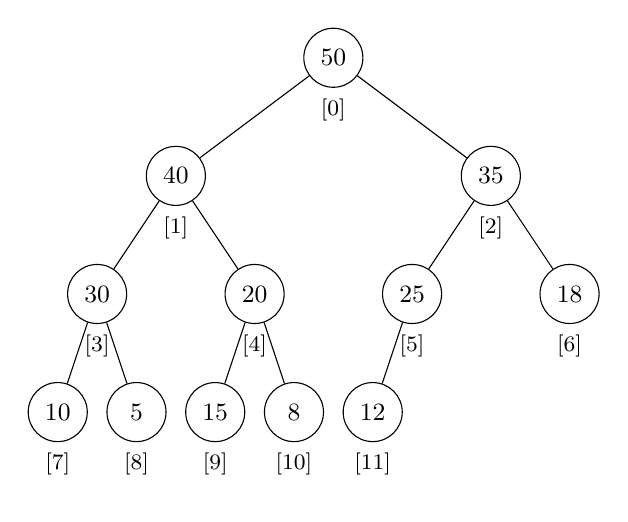
\begin{tikzpicture}[
                level distance=1.5cm, % 层与层之间的距离
                level 1/.style={sibling distance=4cm}, % 第一层节点之间的距离
                level 2/.style={sibling distance=2cm}, % 第二层节点之间的距离
                level 3/.style={sibling distance=1cm}, % 第三层节点之间的距离
                every node/.style={
                    circle, % 圆形节点
                    draw, % 绘制边框
                    minimum size=0.75cm, % 最小大小
                    inner sep=0, % 内边距为 0
                    font=\small % 字体大小
                }
            ]
            
            % 绘制大根堆的二叉树结构
            \node(0) {50} % 根节点
                child {
                    node(1) {40} % 左子节点
                    child {
                        node(3) {30} % 左子节点的左子节点
                        child { node(7) {10} }
                        child { node(8) {5} }
                    }
                    child {
                        node(4) {20} % 左子节点的右子节点
                        child { node(9) {15} }
                        child { node(10) {8} }
                    }
                }
                child {
                    node(2) {35} % 右子节点
                    child {
                        node(5) {25} % 右子节点的左子节点
                        child { node(11) {12} }
                        child [missing]
                    }
                    child { node(6) {18} }
                };
    
                \foreach \i in {0, ..., 11} {
                    \node [font=\footnotesize, below = -0.1cm of \i, draw=none] {[\i]};
                }
            \end{tikzpicture}
        \end{figure}
    \end{frame}

    \subsection{Implementation}

    \begin{frame}{Implementation}{Find parent and child nodes}
        \begin{algorithm}[H]
            \caption{Find parent and child nodes}
            \label{algo:Find parent and child nodes}
            \SetKwFunction{Parent}{Parent}
            \Function{\Parent{$i$}}{
                \Return{$\lfloor (i-1)/2\rfloor$}
            }
    
            \BlankLine
    
            \SetKwFunction{LeftChild}{Left-Child}
            \Function{\LeftChild{$i$}}{
                \Return{$2i+1$}
            }
    
            \BlankLine
    
            \SetKwFunction{RightChild}{Right-Child}
            \Function{\RightChild{$i$}}{
                \Return{$2i+2$}
            }
        \end{algorithm}
    \end{frame}

    \begin{frame}{Implementation}{Insert a new item}
        When inserting a new item into a max-heap, we add it to the end of the array and then \highlight{float} it up to maintain the max-heap property. During this process, the new item is swapped with its parent until the max-heap property is satisfied.

        The time complexity of inserting a new item is $\mathcal O(\log n)$.
    \end{frame}

    \begin{frame}{Implementation}{Insert a new item: Example}
        \begin{figure}[!htbp]
            \centering
            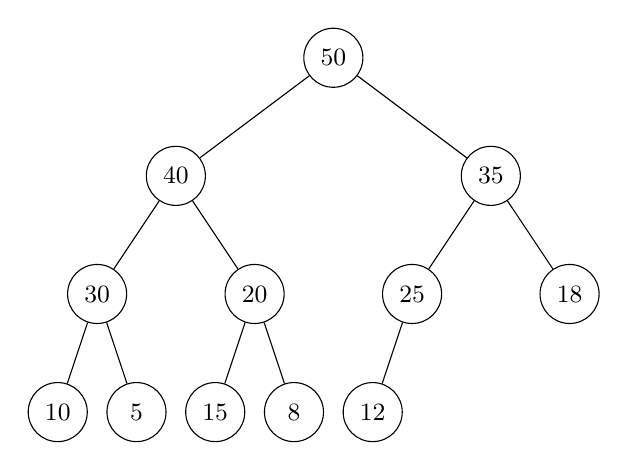
\begin{tikzpicture}[
                level distance=1.5cm,
                level 1/.style={sibling distance=4cm},
                level 2/.style={sibling distance=2cm},
                level 3/.style={sibling distance=1cm},
                every node/.style={
                    circle,
                    draw,
                    minimum size=0.75cm,
                    inner sep=0,
                    font=\small
                }
            ]
            % 初始大根堆
            \node {50}
                child {
                    node {40}
                    child {
                        node {30}
                        child { node {10} }
                        child { node {5} }
                    }
                    child {
                        node {20}
                        child { node {15} }
                        child { node {8} }
                    }
                }
                child {
                    node {35}
                    child {
                        node {25}
                        child { node {12} }
                        child[missing]
                    }
                    child { node {18} }
                };
            \end{tikzpicture}
        \end{figure}
    \end{frame}

    \begin{frame}{Implementation}{Insert a new item: Example}
        \begin{figure}
            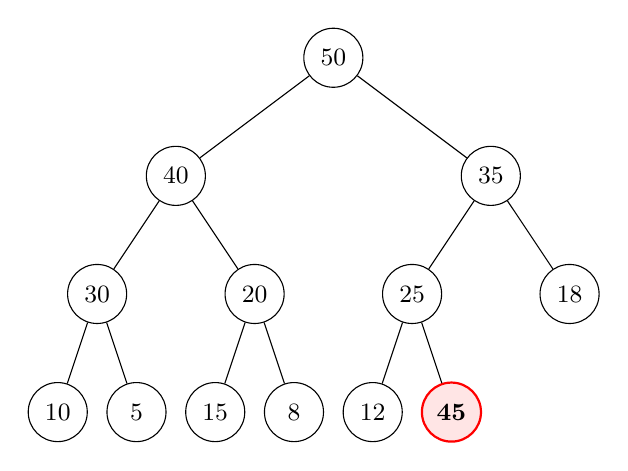
\begin{tikzpicture}[
                level distance=1.5cm,
                level 1/.style={sibling distance=4cm},
                level 2/.style={sibling distance=2cm},
                level 3/.style={sibling distance=1cm},
                every node/.style={
                    circle,
                    draw,
                    minimum size=0.75cm,
                    inner sep=0,
                    font=\small
                }
            ]
            % 初始大根堆
            \node {50}
                child {
                    node {40}
                    child {
                        node {30}
                        child { node {10} }
                        child { node {5} }
                    }
                    child {
                        node {20}
                        child { node {15} }
                        child { node {8} }
                    }
                }
                child {
                    node {35}
                    child {
                        node {25}
                        child { node {12} }
                        child { node[rednode] {45} }
                    }
                    child { node {18} }
                };
            \end{tikzpicture}
        \end{figure}
    \end{frame}

    \begin{frame}{Implementation}{Insert a new item: Example}
        \begin{figure}
            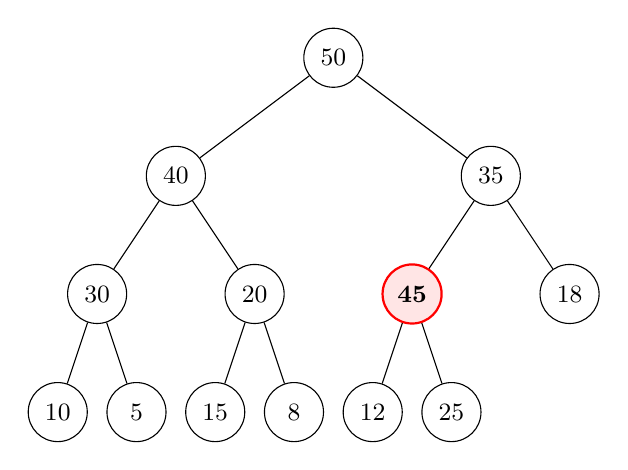
\begin{tikzpicture}[
                level distance=1.5cm,
                level 1/.style={sibling distance=4cm},
                level 2/.style={sibling distance=2cm},
                level 3/.style={sibling distance=1cm},
                every node/.style={
                    circle,
                    draw,
                    minimum size=0.75cm,
                    inner sep=0,
                    font=\small
                }
            ]
            % 初始大根堆
            \node {50}
                child {
                    node {40}
                    child {
                        node {30}
                        child { node {10} }
                        child { node {5} }
                    }
                    child {
                        node {20}
                        child { node {15} }
                        child { node {8} }
                    }
                }
                child {
                    node {35}
                    child {
                        node[rednode] {45}
                        child { node {12} }
                        child { node {25} }
                    }
                    child { node {18} }
                };
            \end{tikzpicture}
        \end{figure}
    \end{frame}

    \begin{frame}{Implementation}{Insert a new item: Example}
        \begin{figure}
            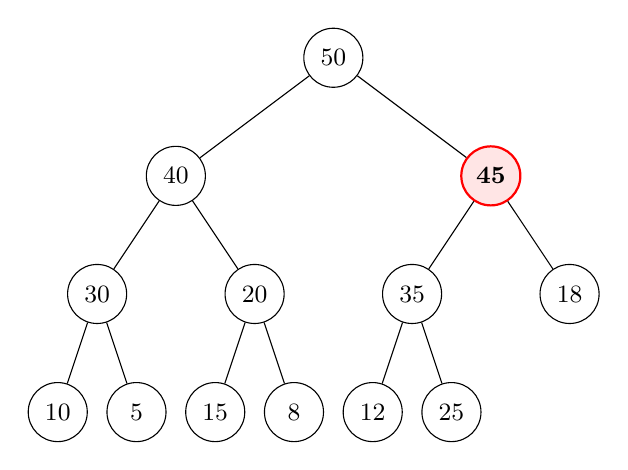
\begin{tikzpicture}[
                level distance=1.5cm,
                level 1/.style={sibling distance=4cm},
                level 2/.style={sibling distance=2cm},
                level 3/.style={sibling distance=1cm},
                every node/.style={
                    circle,
                    draw,
                    minimum size=0.75cm,
                    inner sep=0,
                    font=\small
                }
            ]
            % 初始大根堆
            \node {50}
                child {
                    node {40}
                    child {
                        node {30}
                        child { node {10} }
                        child { node {5} }
                    }
                    child {
                        node {20}
                        child { node {15} }
                        child { node {8} }
                    }
                }
                child {
                    node[rednode] {45}
                    child {
                        node {35}
                        child { node {12} }
                        child { node {25} }
                    }
                    child { node {18} }
                };
            \end{tikzpicture}
        \end{figure}
    \end{frame}

    \begin{frame}{Implementation}{Insert a new item: Algorithm}
        \begin{algorithm}[H]
            \caption{Add a new item to a max-heap}
            \label{algo:Add a new item to a max-heap}
            \SetKwFunction{Insert}{Insert}
            \SetKwFunction{FloatUp}{Float-Up}
            \Function{\Insert{$A,x$}}{
                \SetKwFunction{Pushback}{Push-back}
                $A.\Pushback(x)$\;
                \FloatUp{$A.\textit{size}-1$}\;
            }
            \BlankLine
            \Function{\FloatUp{$i$}}{
                \While{$i > 0$ and $A[i] > A[\Parent{$i$}]$}{
                    Swap $A[i]$ and $A[\Parent{$i$}]$\;
                    $i \gets \Parent{$i$}$\;
                }
            }
        \end{algorithm}
    \end{frame}

    \begin{frame}{Implementation}{Delete the highest-priority item}
        When deleting the highest-priority item from a max-heap, we first swap the root with the last item in the array, then \highlight{sink} the new root down to keep the max-heap property. The \highlight{sink-down} operation is similar to the \highlight{float-up} operation, but we swap the current node with its larger child until the max-heap property is satisfied.

        The time complexity of deleting the highest-priority item is $\mathcal O(\log n)$.
    \end{frame}

    \begin{frame}{Implementation}{Delete the highest-priority item: Example}
        \begin{figure}
            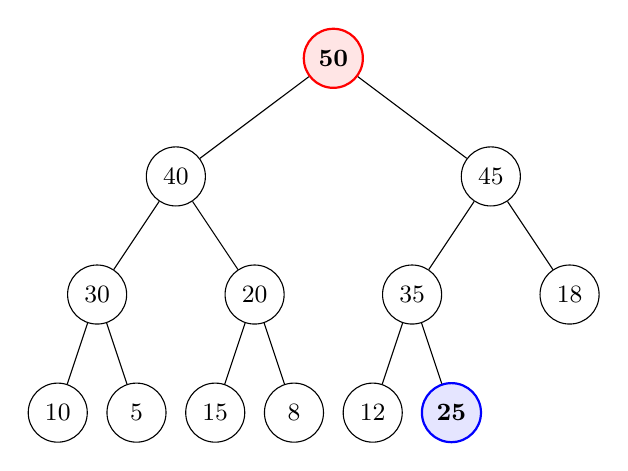
\begin{tikzpicture}[
                level distance=1.5cm,
                level 1/.style={sibling distance=4cm},
                level 2/.style={sibling distance=2cm},
                level 3/.style={sibling distance=1cm},
                every node/.style={
                    circle,
                    draw,
                    minimum size=0.75cm,
                    inner sep=0,
                    font=\small
                }
            ]
            % 初始大根堆
            \node[rednode] {50}
                child {
                    node {40}
                    child {
                        node {30}
                        child { node {10} }
                        child { node {5} }
                    }
                    child {
                        node {20}
                        child { node {15} }
                        child { node {8} }
                    }
                }
                child {
                    node {45}
                    child {
                        node {35}
                        child { node {12} }
                        child { node[bluenode] {25} }
                    }
                    child { node {18} }
                };
            \end{tikzpicture}
        \end{figure}
    \end{frame}

    \begin{frame}{Implementation}{Delete the highest-priority item: Example}
        \begin{figure}
            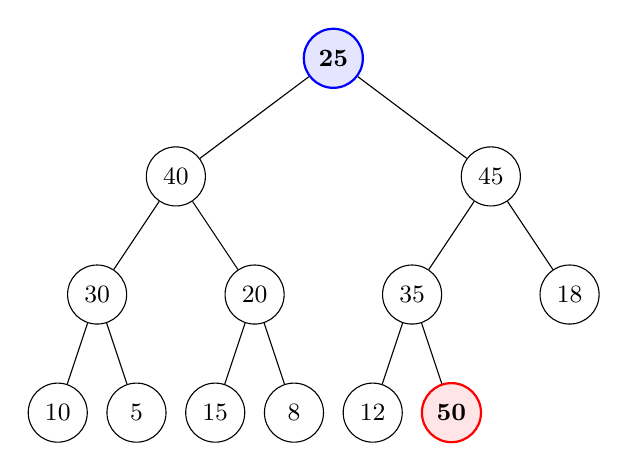
\begin{tikzpicture}[
                level distance=1.5cm,
                level 1/.style={sibling distance=4cm},
                level 2/.style={sibling distance=2cm},
                level 3/.style={sibling distance=1cm},
                every node/.style={
                    circle,
                    draw,
                    minimum size=0.75cm,
                    inner sep=0,
                    font=\small
                }
            ]
            % 初始大根堆
            \node[bluenode] {25}
                child {
                    node {40}
                    child {
                        node {30}
                        child { node {10} }
                        child { node {5} }
                    }
                    child {
                        node {20}
                        child { node {15} }
                        child { node {8} }
                    }
                }
                child {
                    node {45}
                    child {
                        node {35}
                        child { node {12} }
                        child { node[rednode] {50} }
                    }
                    child { node {18} }
                };
            \end{tikzpicture}
        \end{figure}
    \end{frame}

    \begin{frame}{Implementation}{Delete the highest-priority item: Example}
        \begin{figure}
            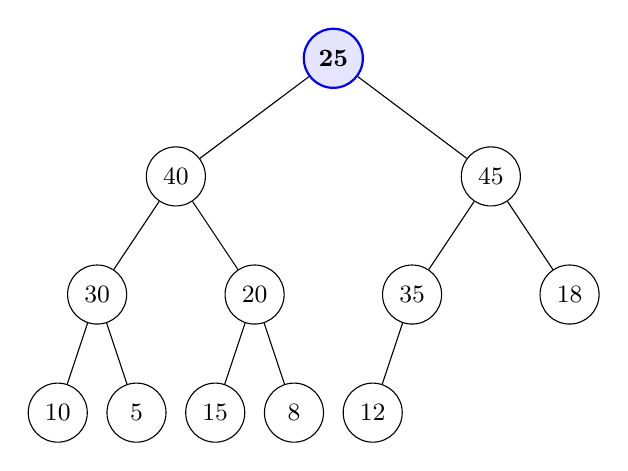
\begin{tikzpicture}[
                level distance=1.5cm,
                level 1/.style={sibling distance=4cm},
                level 2/.style={sibling distance=2cm},
                level 3/.style={sibling distance=1cm},
                every node/.style={
                    circle,
                    draw,
                    minimum size=0.75cm,
                    inner sep=0,
                    font=\small
                }
            ]
            % 初始大根堆
            \node[bluenode] {25}
                child {
                    node {40}
                    child {
                        node {30}
                        child { node {10} }
                        child { node {5} }
                    }
                    child {
                        node {20}
                        child { node {15} }
                        child { node {8} }
                    }
                }
                child {
                    node {45}
                    child {
                        node {35}
                        child { node {12} }
                        child[missing]
                    }
                    child { node {18} }
                };
            \end{tikzpicture}
        \end{figure}
    \end{frame}

    \begin{frame}{Implementation}{Delete the highest-priority item: Example}
        \begin{figure}
            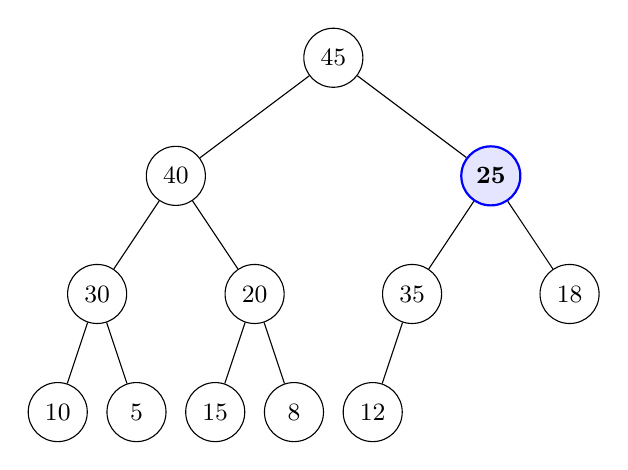
\begin{tikzpicture}[
                level distance=1.5cm,
                level 1/.style={sibling distance=4cm},
                level 2/.style={sibling distance=2cm},
                level 3/.style={sibling distance=1cm},
                every node/.style={
                    circle,
                    draw,
                    minimum size=0.75cm,
                    inner sep=0,
                    font=\small
                }
            ]
            \node {45}
                child {
                    node {40}
                    child {
                        node {30}
                        child { node {10} }
                        child { node {5} }
                    }
                    child {
                        node {20}
                        child { node {15} }
                        child { node {8} }
                    }
                }
                child {
                    node[bluenode] {25}
                    child {
                        node {35}
                        child { node {12} }
                        child [missing]
                    }
                    child { node {18} }
                };
            \end{tikzpicture}
        \end{figure}
    \end{frame}

    \begin{frame}{Implementation}{Delete the highest-priority item: Example}
        \begin{figure}
            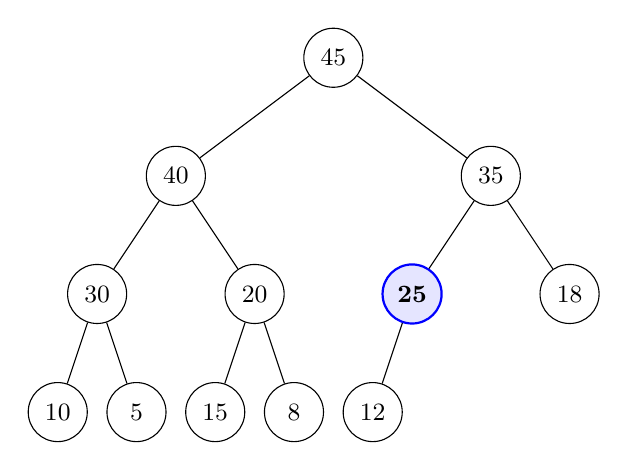
\begin{tikzpicture}[
                level distance=1.5cm,
                level 1/.style={sibling distance=4cm},
                level 2/.style={sibling distance=2cm},
                level 3/.style={sibling distance=1cm},
                every node/.style={
                    circle,
                    draw,
                    minimum size=0.75cm,
                    inner sep=0,
                    font=\small
                }
            ]
            \node {45}
                child {
                    node {40}
                    child {
                        node {30}
                        child { node {10} }
                        child { node {5} }
                    }
                    child {
                        node {20}
                        child { node {15} }
                        child { node {8} }
                    }
                }
                child {
                    node {35}
                    child {
                        node[bluenode] {25}
                        child { node {12} }
                        child [missing]
                    }
                    child { node {18} }
                };
            \end{tikzpicture}
        \end{figure}
    \end{frame}

    \begin{frame}{Implementation}{Delete the highest-priority item: Algorithm}
        \footnotesize
        \begin{algorithm}[H]
            \caption{Delete the highest-priority item from a max-heap}
            \label{algo:Delete the highest-priority item from a max-heap}
    
            \SetKwFunction{Delete}{Delete}
            \SetKwFunction{SinkDown}{Sink-Down}
            \Function{\Delete{$A$}}{
                \SetKwFunction{Popback}{Pop-back}
                Swap $A[0]$ and $A[A.\textit{size}-1]$\;
                $A.\Popback()$\;
                \SinkDown{$A,0$}\;
            }
            
            \BlankLine
    
            \Function{\SinkDown{$A,i$}}{
                \While{$\LeftChild{i} < A.\textit{size}$}{
                    $j \gets \LeftChild{i}$\;
                    \lIf{$j+1 < A.\textit{size}$ and $A[j+1] > A[j]$}{$j \gets j+1$}
                    \lIf{$A[i] \geq A[j]$}{\Return}
                    Swap $A[i]$ and $A[j]$\;
                    $i \gets j$\;
                }
            }
        \end{algorithm}
    \end{frame}

    \begin{frame}{Implementation}{Build a heap from an (unsorted) array}
        When building a heap from an (unsorted) array, we can perform the \highlight{sink-down} operation from the last non-leaf node to the root. After each operation, the subtree rooted at the current node satisfies the max-heap property.

        \begin{algorithm}[H]
            \caption{Build a heap from an (unsorted) array}
            \label{algo:Build a heap from an (unsorted) array}

            \SetKwFunction{BuildHeap}{Build-Heap}
            \SetKw{KwDownTo}{downto}
            \Function{\BuildHeap{$A$}}{
                \For{$i \gets \lfloor A.\textit{size}/2\rfloor-1$ \KwDownTo $0$}{
                    \SinkDown{$A,i$}\;
                }
            }
        \end{algorithm}

        {\bf Remark. }The node with index $i$ has a child iff $\LeftChild{i} < A.\textit{size}$, i.e. $2i+1<A.\textit{size}$. Hence $i\leq\lfloor A.\textit{size}/2\rfloor-1$.
    \end{frame}

    \begin{frame}{Implementation}{Build a heap from an (unsorted) array: Time complexity}
        We consider a complete binary tree with depth $N$ and $n=2^{N+1}-1$ nodes. The number of operation we need when building a heap is
        $$\sum_{i=0}^{N-1}2^i(N-i)=2^{N+1}-N-2=\mathcal O(n).$$
        Therefore, the time complexity of building a heap from an (unsorted) array is $\mathcal O(n)$. We should {\bf NOT} build a heap by inserting items one by one, which takes $\mathcal O(n\log n)$ time.
    \end{frame}

    \begin{frame}[fragile]{Implementation}{Priority queue in C++ STL}
        A \highlight{priority queue} in C++ STL is implemented by a heap. We can define a priority queue of integers by codes below:

        \begin{lstlisting}
#include <queue>

priority_queue<int> pq;                   // max-heap
priority_queue<int, greater<int>> pq_min; // min-heap
        \end{lstlisting}
    \end{frame}

    \begin{frame}{Implementation}{Priority queue in C++ STL}
        Common operations of a priority queue are listed in Table \ref{tab:Operations of a priority queue in C++ STL}.

        \begin{table}[!htbp]
            \centering
            \begin{tabular}{ccc}
                \toprule
                Operation & Description & Time complexity \\
                \midrule
                \texttt{pq.push(x)} & Insert a new item $x$ & $\mathcal O(\log n)$ \\
                \texttt{pq.pop()} & Delete the highest-priority item & $\mathcal O(\log n)$ \\
                \texttt{pq.top()} & Return the highest-priority item & $\mathcal O(1)$ \\
                \bottomrule
            \end{tabular}
            \caption{Operations of a priority queue in C++ STL}
            \label{tab:Operations of a priority queue in C++ STL}
        \end{table}
    \end{frame}

    \begin{frame}{Example: \href{https://www.luogu.com.cn/problem/P1801}{[Luogu] P1801}}{Description}
        A \highlight{black box} is a rudimentary form of database which stores an array of intergers and a special variable $i$. At the beginning, the array is empty and $i=0$. The black box supports the following operations:

        \begin{itemize}
            \item \texttt{ADD(x)}: Add $x$ to the black box.
            \item \texttt{GET}: $i$ increases by 1, and return the $i$-th smallest number in the array.
        \end{itemize}

        Now you are required to find a best way to process a given sequence of operations. The sequence includes $n\ (n\leq 2\times 10^5)$ \texttt{ADD} operations and $m\ (m\leq 2\times 10^5)$ \texttt{GET} operations. Two arrays of interger are used to describe the operation sequence:

        \begin{itemize}
            \item $a_1,a_2,\dots,a_n$: a sequence of integers to be added to the black box. $|a_i|\leq 10^9$.
            \item $u_1,u_2,\dots,u_m$: a \texttt{GET} operation is performed when the $u_i$-th number is added to the black box. $\{u_i\}$ is non-decreasing. No illegal operation will be contained in the sequence.
        \end{itemize}
    \end{frame}

    \begin{frame}{Example: \href{https://www.luogu.com.cn/problem/P1801}{[Luogu] P1801}}{Solution}
        We can use a max-heap to maintain the smallest $i$ numbers, and a min-heap to maintain the rest numbers.
    
        \begin{itemize}
            \item When a new number is added:
            \begin{itemize}
                \item If the number is smaller than the top of the max-heap, we add it to the max-heap, and move the top of the max-heap to the min-heap.
                \item Otherwise, we add it to the min-heap.
            \end{itemize}
            \item When a \texttt{GET} operation is performed, we move the top of the min-heap to the max-heap, and print it.
        \end{itemize}

        The time complexity of each operation is $\mathcal O(\log n)$, so the total time complexity is $\mathcal O((n+m)\log n)$.
    \end{frame}

    \section{Disjoint-set forests}

    \begin{frame}{Disjoint-set}{Definition}
        A \highlight{disjoint-set} data structure maintains a collection of disjoint sets, each of which is represented by a unique \highlight{representative}. We can perform the following operations on disjoint sets:

        \begin{itemize}
            \item \textsc{Make-Set}$(x)$: create a new set containing $x$.
            \item \textsc{Union}$(x,y)$: merge the sets containing $x$ and $y$.
            \item \textsc{Find}$(x)$: find the representative of the set containing $x$.
            \item \textsc{Is-Same}$(x,y)$: check whether $x$ and $y$ are in the same component.
        \end{itemize}
    \end{frame}

    \begin{frame}{Disjoint-set forests}{Disjoint-set forests}
        A fast implementation of disjoint-set is \highlight{disjoint-set forests}. We represent each set as a \highlight{tree}, where the representative is the \highlight{root} of the tree.

        A \textsc{Make-Set} operation creates a tree with a single node. A \textsc{Union} operation merges two trees by making the root of one tree a child of the root of the other tree. A \textsc{Find} operation returns the root of the tree containing $x$.
    \end{frame}

    \begin{frame}{Disjoint-set forests}{Example}
        \begin{figure}[!htbp]
            \centering
            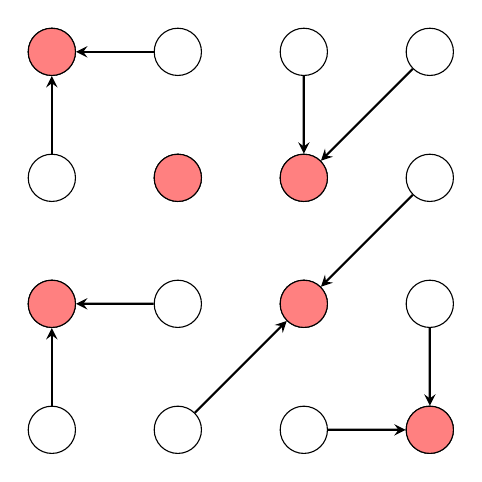
\begin{tikzpicture}[
                scale=0.8,
                node/.style={circle, draw, minimum size=0.6cm, fill=white},
                root/.style={circle, draw, minimum size=0.6cm, fill=red!50},
                edge/.style={->, >=stealth, thick}
            ]
                % 定义节点
                \foreach \i in {0, 1, 2, 3} {
                    \foreach \j in {0, 1, 2, 3} {
                        \node[node] (\i\j) at (2*\i, -2*\j) {};
                    }
                }
            
                % 设置根节点并染色
                \node[root] (00) at (0, 0) {};    % 连通块 1 的根
                \node[root] (21) at (4, -2) {};    % 连通块 2 的根
                \node[root] (02) at (0, -4) {};   % 连通块 3 的根
                \node[root] (22) at (4, -4) {};   % 连通块 4 的根
                \node[root] (33) at (6, -6) {};   % 连通块 5 的根
                \node[root] (11) at (2, -2) {};
            
                % 连接边形成树,确保连线不跨过其他节点
                % 连通块 1
                \draw[edge] (10) -- (00); % 1,0 -> 0,0
                \draw[edge] (01) -- (00); % 0,1 -> 0,0
            
                % 连通块 2
                \draw[edge] (20) -- (21);
                \draw[edge] (30) -- (21);
            
                % 连通块 3
                \draw[edge] (12) -- (02); % 1,2 -> 0,2
                \draw[edge] (03) -- (02); % 0,3 -> 0,2
            
                % 连通块 4
                \draw[edge] (32) -- (33); % 3,2 -> 2,2
                \draw[edge] (23) -- (33); % 2,3 -> 2,2
            
                % 连通块 5
                \draw[edge] (13) -- (22);
                \draw[edge] (31) -- (22);
            
            \end{tikzpicture}
        \end{figure}
    \end{frame}

    \begin{frame}{Disjoint-set forests}{Heuristics to improve efficiency}
        \begin{itemize}
            \item {\bf Union by rank}: we attach the tree with smaller \highlight{rank} to the tree with larger rank. Here the rank of a node is the height of the subtree rooted at the node.
            \item {\bf Path compression}: when we find the root of the tree containing $x$, we make all the nodes on the path from $x$ to the root point directly to the root.
        \end{itemize}
    
        With both heuristics, the time complexity of each operation is $\mathcal O(\alpha(n))$, where $n$ is the number of elements and $\alpha(\cdot)$ is the \highlight{inverse Ackermann function}. The function grows very slowly, so we can consider it as a constant.
    \end{frame}

    \begin{frame}{Disjoint-set forests}{Algorithm}
        \small
        \begin{algorithm}[H]
            \caption{Disjoint-set forests}
            \SetKwFunction{MakeSet}{Make-Set}
            \SetKwFunction{Find}{Find}
            \SetKwFunction{Union}{Union}
            \SetKwFunction{Link}{Link}
            \Function{\MakeSet{$x$}}{
                $\textit{parent}[x] \gets x$\;
                $\textit{rank}[x] \gets 0$\;
            }
    
            \BlankLine
    
            \Function{\Find{$x$}}{
                \lIf{$x\neq\textit{parent}[x]$}{$\textit{parent}[x] \gets \Find{\textit{parent}[$x$]}$}
                \Return{$\textit{parent}[x]$}\;
            }
    
            \BlankLine

            \SetKwFunction{IsSame}{Is-Same}

            \Function{\IsSame{$x,y$}}{
                \Return{$\Find{x} = \Find{y}$}\;
            }
        \end{algorithm}
    \end{frame}

    \begin{frame}{Disjoint-set forests}{Algorithm}
        \small
        \begin{algorithm}[H]
            \caption{Disjoint-set forests}
            \SetKwFunction{MakeSet}{Make-Set}
            \SetKwFunction{Find}{Find}
            \SetKwFunction{Union}{Union}
            \SetKwFunction{Link}{Link}
            \Function{\Link{$x,y$}}{
                \lIf{$\textit{rank}[x] > \textit{rank}[y]$}{$\textit{parent}[y] \gets x$}
                \Else{
                    $\textit{parent}[x] \gets y$\;
                    \If{$\textit{rank}[x] = \textit{rank}[y]$}{
                        $\textit{rank}[y] \gets \textit{rank}[y]+1$\;
                    }
                }
            }

            \BlankLine
    
            \Function{\Union{$x,y$}}{
                $x \gets \Find{x}$, $y \gets \Find{y}$\;
                \lIf{$x\neq y$}{\Link{$x,y$}}
            }
        \end{algorithm}
    \end{frame}

    \begin{frame}{Application: Kruskal's algorithm}{Minimum spanning tree \& Kruskal's algorithm}
        A \highlight{minimum spanning tree} of a connected, undirected graph is a spanning tree with the smallest possible sum of edge weights. A minimum spanning tree is unique if the edge weights are distinct.

        \highlight{Kruskal's algorithm} is a greedy algorithm that finds a minimum spanning tree for a connected, undirected graph. In each iteration, the algorithm finds the edge with the smallest weight which links two different components, and adds it to the minimum spanning tree. We repeat this process until all the vertices are connected.
    \end{frame}

    \begin{frame}{Application: Kruskal's algorithm}{Algorithm}
        \footnotesize
        \begin{algorithm}[H]
            \caption{Kruskal's algorithm}
            \label{algo:Kruskal's algorithm}
    
            \SetKwFunction{Kruskal}{Kruskal}
            \SetKwFunction{MakeSet}{Make-Set}
            \SetKwFunction{Find}{Find}
            \SetKwFunction{Union}{Union}
            \SetKwFunction{IsSame}{Is-Same}
            \SetKwData{false}{false}
    
            \Function{\Kruskal{$G$}}{
                Sort $G.\textit{edges}$ by weight in non-decreasing order\;
                \For{$v\in G.\textit{vertices}$}{
                    \MakeSet{$v$}\;
                }
                $T \gets \varnothing$\;
                \For{$e\in G.\textit{edges}$}{
                    \If{$\IsSame{e.\textit{from}, e.\textit{to}}=\false$}{
                        $T \gets T\cup\{e\}$\;
                        \Union{$e.\textit{from},e.\textit{to}$}\;
                    }
                }
                \Return{$T$}\;
            }
        \end{algorithm}
    \end{frame}

    \appendix

    \begin{frame}
        \calligra \centering
        \scalebox{3}{
            Thanks for your attention!
        }
    \end{frame}
\end{document}